\chapter{Implementation}
\label{sec:implementation}

This chapter describes the system as it was built and run. The graph of
Figure~\ref{fig:graph} was implemented node for node in LangGraph~\cite{langgraph};
where the implementation departs from the original design, the reason is given.

\section{Software and Hardware}

Table~\ref{tab:stack} lists the components. Everything ran on one desktop PC with a
consumer GPU (Intel Arc B580, 12~GB) and 15.6~GB of RAM, fully offline: every model
was loaded from a local copy, and no evaluation depended on a paid service.

\begin{table}[htbp]
\centering
\small
\begin{tabular}{lp{8.6cm}}
\toprule
Component & Choice \\
\midrule
Agent framework & LangGraph (Python 3.12), one node per box of Figure~\ref{fig:graph} \\
PDF reading & PyMuPDF~\cite{pymupdf}: text layer, page images (150~dpi), vector charts \\
Table structure & Table Transformer~\cite{smock2022pubtables} \\
Text index & SPECTER2~\cite{singh2023scirepeval} (768-d) in FAISS~\cite{johnson2019faiss}, fused with keyword search \\
Page index & ColQwen2~\cite{faysse2025colpali}, 128-d vectors per page patch \\
Language model & Qwen2.5-VL-7B-Instruct~\cite{bai2025qwen25vl}, 4-bit (Q4\_K\_M), llama.cpp~\cite{llamacpp} server \\
Comparison model & Gemini 3.5 Flash-Lite (free tier), through the same request format \\
\bottomrule
\end{tabular}
\caption{The software stack.}
\label{tab:stack}
\end{table}

\section{Ingestion and Indexing (N3, N4)}

Each paper is read once, offline. Its text is split into paragraphs; its tables and
figures are located with their captions and bounding boxes; every table is parsed
into cells, each with its own page coordinates; and bar charts drawn as vector
graphics are read directly from the PDF, so that a bar's value and position are
exact rather than estimated from pixels. Two indexes are built: SPECTER2 vectors of
the paragraphs in FAISS, and ColQwen2 patch vectors of every page image. Only one
large model fits on the 12~GB GPU at a time, so the page index is built before the
language model is started, and at question time ColQwen2 runs only from cached
question vectors.

\section{The Language Model in the Loop}

The model serves six roles: splitting the question into sub-goals and naming the
entities it is about (N1, N2), planning the next tool (N5), judging sufficiency (G1),
writing the answer (N9), and checking each claim's support (G2). Every call follows
the same pattern:

\begin{itemize}
    \item The reply is forced into a JSON schema by the server's grammar, so it can
    always be parsed. Temperature is 0 and the seed is fixed.
    \item Every reply is cached under a hash of the full request, and the cache is
    kept under version control. A re-run reproduces every answer exactly, and a power
    cut never costs more than the question in progress.
    \item Every reply is capped (2{,}048 tokens, and length limits inside the schema):
    the 7B model once repeated itself for 5{,}800 tokens inside one field.
    \item If the model cannot be reached or replies without the required fields, the
    node falls back to a simple rule and the trace records it. Across all test runs,
    four questions used a fallback.
\end{itemize}

Two design details mattered more than expected. First, \textbf{the Sufficiency Gate
writes its facts before its verdict}. llama.cpp fills the fields of a JSON reply in
schema order, so a verdict written first was only justified afterwards; with the
order reversed, the gate must name the fact that answers the question before
declaring sufficiency. Second, \textbf{the kind of evidence a sub-goal needs} (table
or figure) is not asked of the model but voted by the nine most similar labelled SPIQA
questions from papers that are in neither split; on the development questions this
chose the reference's kind 17 times out of 20, against 8 for the model.

\section{Generation and Verification (N9, G2)}

The writer receives the evidence buffer --- paragraphs, parsed tables as cells, and
figure images --- and must return a list of claims, each citing its evidence: a
verbatim quote, a table cell (row, column, value), or an observation about a figure.
The Faithfulness Gate checks every claim in two layers:

\begin{enumerate}
    \item \textbf{Exact check.} A quote must occur in the cited paragraph, and a cell
    value must equal the parsed cell. Both sides are first normalised for the quirks
    of PDF text extraction (ligatures, line-end hyphenation, spaced decimals such as
    ``0 . 5'', curly quotes); without this, four of the twenty development questions
    lost a correct claim. A changed word or number still fails.
    \item \textbf{Support check.} The model judges whether the cited evidence
    supports the claim as written, which catches a correct quote attached to a wrong
    conclusion.
\end{enumerate}

\noindent A failed claim sends the draft back with the reason, at most twice. Claims
still failing are withheld and listed as unconfirmed; if every claim fails, the
answer says that nothing can be stated.

\section{Exact Proof Boxes (N10b)}

Every published claim receives a box on the page, chosen in this order: the cited
table cell; the bar of a vector chart; the quoted sentence, found on the page (even
when split across lines); the caption; the labels inside a diagram that the
observation names; and, only for photographs, the box around the highest-scoring
patches of ColQwen2's similarity map. For the photograph case, a second pass after
the evaluation computed the map for each claim's own text rather than for the
question, from cached vectors; 78 claims across the five runs were re-boxed this way,
without any change to the answers. Figure~\ref{fig:grounded-answer} shows an output.

\begin{figure}[htbp]
\centering
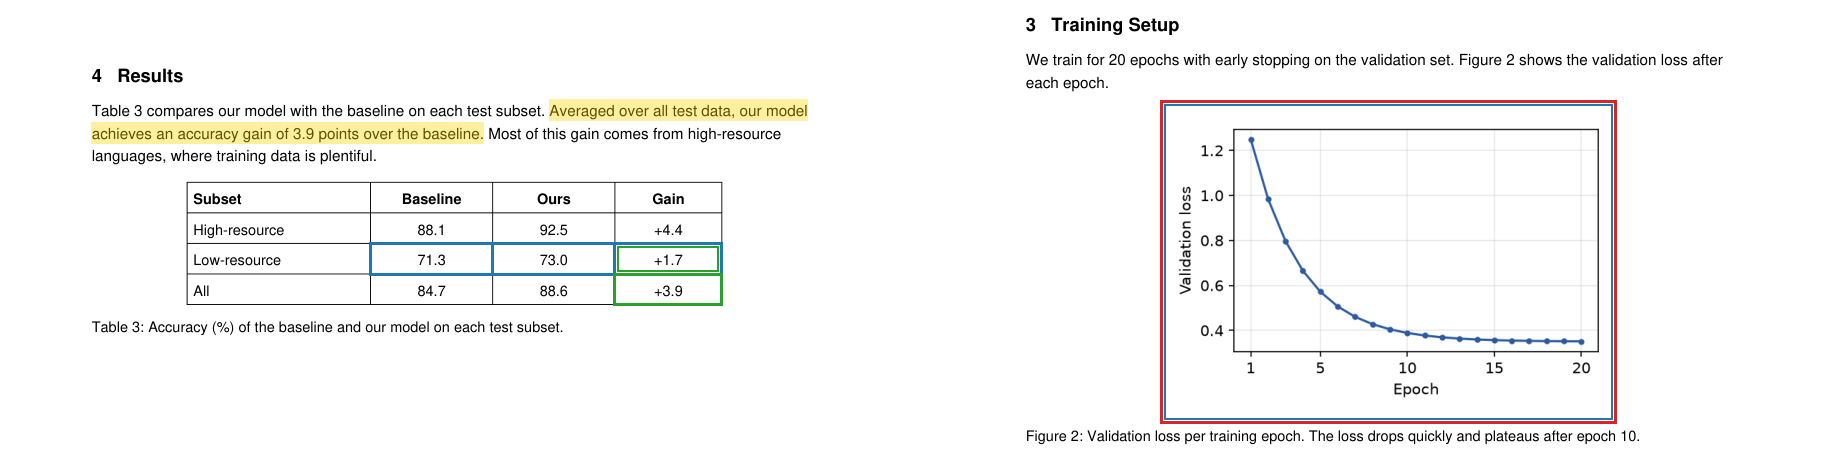
\includegraphics[width=0.85\linewidth]{figures/fig_grounded_answer.png}
\caption{A grounded answer: each claim's proof box drawn on the source page.}
\label{fig:grounded-answer}
\end{figure}

\section{Evaluation Runner and Power-Cut Safety}

The evaluation ran on a shared PC under daily power cuts, so the runner was built to
survive them. Each finished question is appended to a file and forced to disk before
the next starts; a restart skips finished questions; a question during which the
model became unreachable is discarded and redone, so no stand-in answer enters the
results; and every expensive file is written under a temporary name and renamed only
when complete. One script restarts everything after a power cut: it starts the model
server when memory and GPU allow, continues each system where it stopped, and
commits the results. On the test split the runner prints no question or answer text
and refuses to start if any setting differs from the frozen configuration.

\section{Design Validation on a Synthetic Paper}

Before any real paper was used, the whole graph ran on a small synthetic paper with
deterministic stand-ins for every model. This tested the control flow of every path
--- one round, a zoom, a rejected buffer, a rewritten draft, a draft that is never
corrected, an unanswerable question --- with exact, repeatable traces
(Table~\ref{tab:execution-profile}, Figure~\ref{fig:execution-trace}). Over 140 automated
tests protect this behaviour.

\begin{table}[htbp]
\centering
\small
% Generated by notebooks/langgraph_demo.ipynb (test 11I).
% Do not edit by hand -- re-run the notebook instead.
\begin{tabular}{@{}lrrrrrr@{}}
\toprule
Scenario & $R$ & $Z$ & $W$ & Steps & Node runs & Model calls \\
\midrule
Text, 1 round & 1 & 0 & 0 & 11 & 13 & 6 \\
Figure, zoom & 1 & 1 & 0 & 12 & 14 & 6 \\
Running example & 2 & 0 & 0 & 16 & 18 & 8 \\
Running ex., 1 misquote & 2 & 0 & 1 & 19 & 21 & 10 \\
Running ex., never corrected & 2 & 0 & 2 & 23 & 25 & 12 \\
Unanswerable & 3 & 0 & 0 & 20 & 20 & 8 \\
Worst case (3 sub-goals) & 3 & 1 & 2 & 29 & 31 & 14 \\
\bottomrule
\end{tabular}

\caption{Execution profile on the synthetic paper. $R$ = retrieval rounds, $Z$ = zooms,
$W$ = rewrites.}
\label{tab:execution-profile}
\end{table}

\begin{figure}[htbp]
\centering
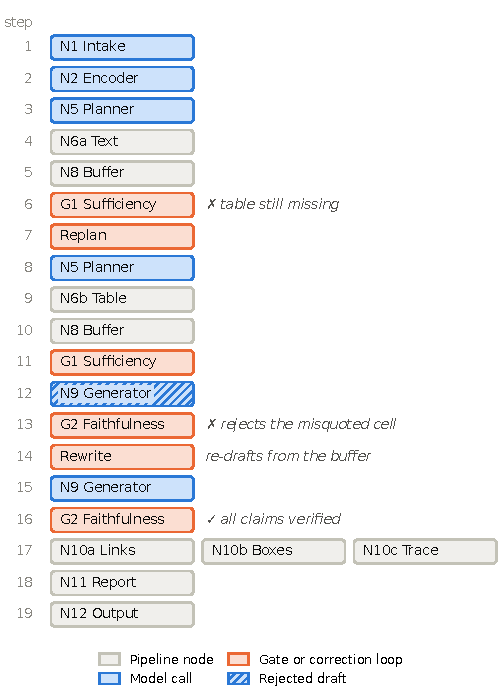
\includegraphics[width=\linewidth]{figures/fig_execution_trace.pdf}
\caption{Execution trace of the running example on the synthetic paper.}
\label{fig:execution-trace}
\end{figure}
